\documentclass[10pt]{article}
\usepackage[polish]{babel}
\usepackage[utf8]{inputenc}
\usepackage[T1]{fontenc}
\usepackage{amsmath}
\usepackage{amsfonts}
\usepackage{amssymb}
\usepackage[version=4]{mhchem}
\usepackage{stmaryrd}
\usepackage{graphicx}
\usepackage[export]{adjustbox}
\graphicspath{ {./images/} }

\title{LIGA MATEMATYCZNA \\
 GRUDZIEŃ 2009 \\
 SZKOŁA PODSTAWOWA }

\author{}
\date{}


\begin{document}
\maketitle
\section*{ZADANIE 1.}
Monia, Tonia, Ponia i Sonia są koleżankami. Dwie z nich są rówieśniczkami. Monia byłaby starsza od Toni, gdyby nie była młodsza od Soni. Ponia byłaby młodsza od Toni, gdyby nie była starsza od Soni. Kto jest rówieśniczką Toni: Ponia, Monia czy Sonia?

\section*{ZADANIE 2.}
Przez stację kolejową przejechały trzy pociągi wojskowe. W pierwszym było 462 żołnierzy, w drugim 546, w trzecim 630. Czy można obliczyć z ilu wagonów składał się każdy z pociągów, jeżeli wiadomo, że w każdym wagonie była jednakowa ilość żołnierzy i że ta liczba była największa ze wszystkich możliwych?

\section*{ZADANIE 3.}
Figura przedstawiona na rysunku składa się z siedmiu kwadratów. Długości boków dwóch spośród tych kwadratów zostały podane. Iloma kwadratami typu \(B\) można wypełnić kwadrat \(A\) ?\\
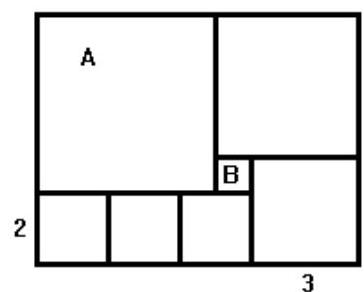
\includegraphics[max width=\textwidth, center]{2024_11_21_5747135af9543a0e0c7fg-1(1)}

\section*{ZADANIE 4.}
Prostokąt podzielono na cztery mniejsze prostokąty. Pola trzech z nich są równe odpowiednio 3,4,5. Jakie jest pole czwartego prostokąta?\\
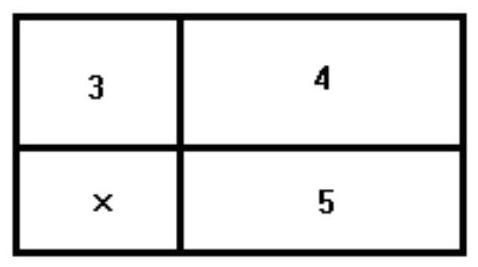
\includegraphics[max width=\textwidth, center]{2024_11_21_5747135af9543a0e0c7fg-1}

\section*{ZADANIE 5.}
Mamy trzy rodzaje patyczków: 16 patyczków o długości 1 cm , 15 patyczków o długości 2 cm i 15 patyczków o długości 3 cm . Czy można zbudować ze wszystkich patyczków prostokąt? Patyczki tworzace boki prostokąta nie mogą zachodzić na siebie i nie można ich łamać.


\end{document}